\section*{Experiment 8: Analysis of the Waveform of the Full Wave Rectifier Circuit}  
\addcontentsline{toc}{section}{Experiment 8: Analysis of the Waveform of the Full Wave Rectifier Circuit}

\subsection*{Learning Objectives:}
\begin{itemize}
    \item Understand the operation of a full wave rectifier circuit.
    \item Analyze the output waveform of a full wave rectifier using an oscilloscope.
\end{itemize}

\subsection*{Equipment:}
\begin{itemize}
    \item Signal Generator (adjustable frequency and amplitude)
    \item Breadboard
    \item Diodes (\verb|1N4001| or similar - 4 required)
    \item Resistor, $R_L$ ($100\Omega, 220\Omega, 470\Omega, 1k\Omega$)
    \item Capacitor, $C$ ($10 \mu F$)
    \item Multimeter (DC voltage measurement)
    \item Oscilloscope
\end{itemize}

\subsection*{Procedure:}

\begin{enumerate}
    \item \textbf{Circuit Construction:} Build the following circuit on the breadboard:

    \begin{itemize}
        \item The full-wave bridge rectifier circuit is composed of four diodes connected in a bridge with no need for a center-tap transformer.
        \item The output of the bridge rectifier is connected to a load resistor (RL) and then to the oscilloscope.
    \end{itemize}

    \item \textbf{Setting Up the Signal Generator:}
    \begin{itemize}
        \item Set the signal generator to output a sinusoidal waveform (AC).

        \begin{figure}[H]
            \centering
            \includesvg[width=0.75\linewidth]{img/full_wave.svg}
            \caption{Full wave bridge rectifier circuit.}
            \label{fig:full_wave}
        \end{figure}

        \item Adjust the amplitude of the output signal to a suitable level (e.g., $5V$ peak-to-peak).

        \item Start with a low frequency (e.g., $50$ Hz).
    \end{itemize}

    \item \textbf{Observing the Waveform:}
    \begin{itemize}
        \item Connect the oscilloscope probes to the input (across point A and C) and output (across the load resistor) of the circuit.
        
        \item Adjust the oscilloscope settings (vertical scale, horizontal scale, and trigger) to obtain a clear view of the waveforms.
    \end{itemize}

    \item \textbf{Analysis:}
    \begin{itemize}
        \item Sketch the input and output waveforms observed on the oscilloscope.
        \item Measure the peak-to-peak voltage of the output waveform.
        \item Verify that the output waveform is rectified (converted to a pulsating DC waveform).
    \end{itemize}

    \item Filtering (if using a capacitor):
    \begin{itemize}
        \item Modify the circuit by adding a capacitor in parallel with the resistor at the output.
        \item Observe the change in the output waveform on the oscilloscope.
        \item Explain how the capacitor affects the rectified waveform.
    \end{itemize}
\end{enumerate}

\subsection*{Data and Calculations:}
\begin{itemize}
    \item Record the measured peak-to-peak voltage of the input and output waveforms.   
    \item Calculate the average DC voltage at the output using a multimeter. The DC voltage at the output is given by

    $$ V_{dc} = 2 \times \frac{V_P - 2V_b} {\pi} $$

    Where, $V_P$ = Peak input voltage and $V_b$ = built-in voltage ($0.7V$ for silicon diode)

    \begin{figure}
        \centering
        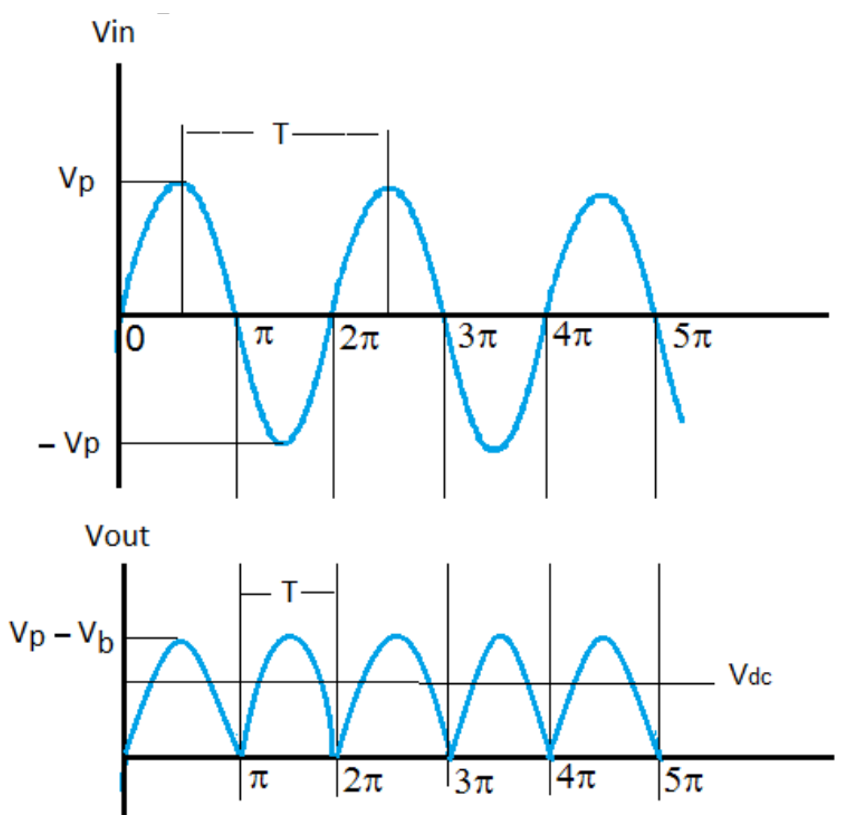
\includegraphics[width=0.5\linewidth]{img/full_wave_form.png}
        \label{fig:full_wave_form}
    \end{figure}

    \item When a voltmeter measures the input voltage, the root-mean-square voltage must satisfy

    $$V_{rms} = \frac{V_P}{\sqrt{2}}$$
\end{itemize}

\subsection*{Observation Table:}

\noindent Without capacitor:
\begin{table}[h]
    \centering
    \begin{tabular}{c|c|c|c|c}
        \hline
        Resistance, $R_L$ & $V_{dc}$ & $V_{rms}$ & $I_{dc} = V_{dc} / R_L$ & $I_{rms} = V_{rms} / R_L$ \\ \hline
         &  &   &    &  \\ \hline
    \end{tabular}
    \label{tab:without_cap}
\end{table}

\noindent With capacitor:
\begin{table}[h]
    \centering
    \begin{tabular}{c|c|c|c|c}
        \hline
        Resistance, $R_L$ & $V_{dc}$ & $V_{rms}$ & $I_{dc} = V_{dc} / R_L$ & $I_{rms} = V_{rms} / R_L$ \\ \hline
         &  &   &    &  \\ \hline
    \end{tabular}
    \label{tab:without_cap}
\end{table}

\subsection*{Conclusion:}
By analyzing the waveforms and DC voltage measurement, verify the operation of the full wave rectifier circuit in converting AC voltage to pulsating DC voltage. Observe how the optional capacitor can help smooth out the rectified waveform.


\newpage